\documentclass[11pt,a4paper]{article}

% ============================================================
% Packages
% ============================================================
\usepackage[margin=2.6cm]{geometry}
\usepackage{amsmath,amssymb,amsthm,mathtools,bm}
\usepackage{booktabs}
\usepackage{microtype}
\usepackage{xcolor}
\usepackage[most]{tcolorbox}
\usepackage{hyperref}
\usepackage{enumitem}
\usepackage{pgfplots}
\pgfplotsset{compat=1.18}
\usepgfplotslibrary{groupplots}
\usepackage{float}

\hypersetup{
  colorlinks=true,
  linkcolor=blue!55!black,
  citecolor=blue!55!black,
  urlcolor=blue!55!black
}

% ============================================================
% Theorem environments (matching the base document)
% ============================================================
\theoremstyle{plain}
\newtheorem{theorem}{Theorem}[section]
\newtheorem{proposition}[theorem]{Proposition}
\newtheorem{lemma}[theorem]{Lemma}
\newtheorem{corollary}[theorem]{Corollary}

\theoremstyle{definition}
\newtheorem{definition}[theorem]{Definition}

\theoremstyle{remark}
\newtheorem{remark}[theorem]{Remark}

\newtcolorbox{keybox}[1][]{
  colback=gray!5,
  colframe=black!45,
  boxrule=0.7pt,
  arc=2pt,
  left=8pt,right=8pt,top=6pt,bottom=6pt,
  fonttitle=\bfseries,
  title={#1}
}

\newtcolorbox{warningbox}[1][]{
  colback=red!3,
  colframe=red!45,
  boxrule=0.7pt,
  arc=2pt,
  left=8pt,right=8pt,top=6pt,bottom=6pt,
  fonttitle=\bfseries,
  title={#1}
}

% ============================================================
% Commands
% ============================================================
\newcommand{\bx}{\bm{x}}
\newcommand{\ba}{\bm{a}}
\newcommand{\br}{\bm{r}}
\newcommand{\be}{\bm{e}}
\newcommand{\bone}{\bm{1}}
\newcommand{\R}{\mathbb{R}}
\newcommand{\E}{\mathbb{E}}
\newcommand{\Prob}{\mathbb{P}}
\newcommand{\norm}[1]{\left\lVert #1\right\rVert}
\newcommand{\Tr}{\operatorname{Tr}}
\newcommand{\lam}{\lambda}
\newcommand{\lsplit}{\lambda_{\mathrm{split}}}
\newcommand{\Lsplit}{\Lambda_{\mathrm{split}}}
\newcommand{\bw}{\beta}
\newcommand{\phib}{\varphi_{\bw}}
\newcommand{\bwc}{\beta_c}

% ============================================================
\title{\bfseries
Bandwidth-Controlled Pareto Differentiation Flow:\\
Full Derivation, Kernel Behaviour, and the Critical Bandwidth $\bwc(\gamma)$
}

\author{Amit Alper\\
\small Hebrew University of Jerusalem\\[2pt]
\small \emph{Supplement to: ``Collective Bifurcations in a Pareto Differentiation Flow''}}
\date{\today}

\begin{document}
\maketitle

\begin{abstract}
We generalize the collective Pareto differentiation flow by introducing an
explicit bandwidth parameter $\bw>0$ into the interaction kernel,
$p(d)=e^{-\bw d^{\gamma}}$, in place of the fixed kernel $e^{-d^\gamma}$ used
previously. We re-derive the deterministic flow, the transverse stability
tensor, and the two-target transverse eigenvalue from scratch with $\bw$ kept
explicit throughout. The bandwidth turns out not to be a cosmetic rescaling:
it introduces a genuine second bifurcation parameter. In particular, for
$\gamma>1$ there is a critical bandwidth
\[
  \bwc(\gamma)=1-\frac{1}{\gamma}
\]
below which the terminal symmetric (Pareto) configuration is transversally
\emph{stable} rather than unstable, and a convexity argument shows this
extends to a complete classification of the transverse stability profile
along the entire trajectory, for every $(\gamma,\bw)$. We also verify that
$\bw$, unlike the population size $N$, cannot be absorbed into a time
rescaling: it moves the bifurcation set itself. Alongside the population,
we give a full stability analysis of a single isolated cell ($N=1$),
including its own transverse eigenvalue, and show it obeys a clean global
dichotomy independent of bandwidth: for $\gamma\ge1$ the single-cell cost is
convex, so \emph{every} trajectory converges to the shared compromise point;
for $\gamma<1$ that point becomes a saddle and every off-axis trajectory
instead reaches a single archetype exactly, in finite time.
\end{abstract}

\tableofcontents

% ============================================================
\section{Notation}
\label{sec:notation}
% ============================================================

\begin{remark}[A notational collision, resolved]
The base document uses the letter $b$ for the half-spacing between the two
side targets in the three-target geometry, $\ba_{1,2}=(\mp b,0)$. To avoid
confusion with that quantity, the new bandwidth parameter introduced here is
denoted $\bw$ (beta) throughout. Wherever both quantities appear together
(Section~\ref{sec:three}), they are visually and semantically distinct:
$b$ is a \emph{geometric} length scale of the target configuration, while
$\bw$ is a \emph{kernel} parameter controlling how sharply the interaction
decays with distance.
\end{remark}

% ============================================================
\section{The bandwidth-modified kernel}
\label{sec:kernel}
% ============================================================

\subsection{Definition}

We replace the interaction kernel of the base model,
\[
  p(d)=e^{-d^{\gamma}},
\]
by the two-parameter family
\begin{equation}
  \boxed{
  p(d)=e^{-\bw d^{\gamma}},
  \qquad \bw>0,\ \gamma>0.
  }
  \label{eq:kernel_def}
\end{equation}
The exponent $\gamma$ still controls the \emph{shape} of the decay
(sub-exponential for $\gamma<1$, exponential at $\gamma=1$, Gaussian-like at
$\gamma=2$, increasingly step-like for large $\gamma$). The new parameter
$\bw$ controls the \emph{scale}: it is a bandwidth in the sense that the
kernel's characteristic width shrinks as $\bw$ grows. Precisely,
\[
  p(d)=e^{-1}
  \quad\Longleftrightarrow\quad
  d=\bw^{-1/\gamma},
\]
so the ``$e$-folding radius'' of the kernel is $\bw^{-1/\gamma}$: larger
$\bw$ means a narrower, more sharply peaked kernel; smaller $\bw$ means a
broader, more permissive one. The original model is recovered at $\bw=1$.

\subsection{How the kernel actually looks}

Figure~\ref{fig:kernel_beta} shows $p(d)=e^{-\bw d^{\gamma}}$ at fixed
$\gamma=2$ for five values of $\bw$: increasing $\bw$ compresses the kernel
toward the origin without changing its qualitative (Gaussian) shape.
Figure~\ref{fig:kernel_gamma} shows the complementary picture: at fixed
$\bw=1$, changing $\gamma$ changes the \emph{shape} of the decay — from a
cusped, heavy-shouldered profile at $\gamma=0.5$, through the exponential
$\gamma=1$ and Gaussian $\gamma=2$ cases, to an increasingly flat-then-cliff
profile as $\gamma$ grows.

\begin{figure}[H]
\centering
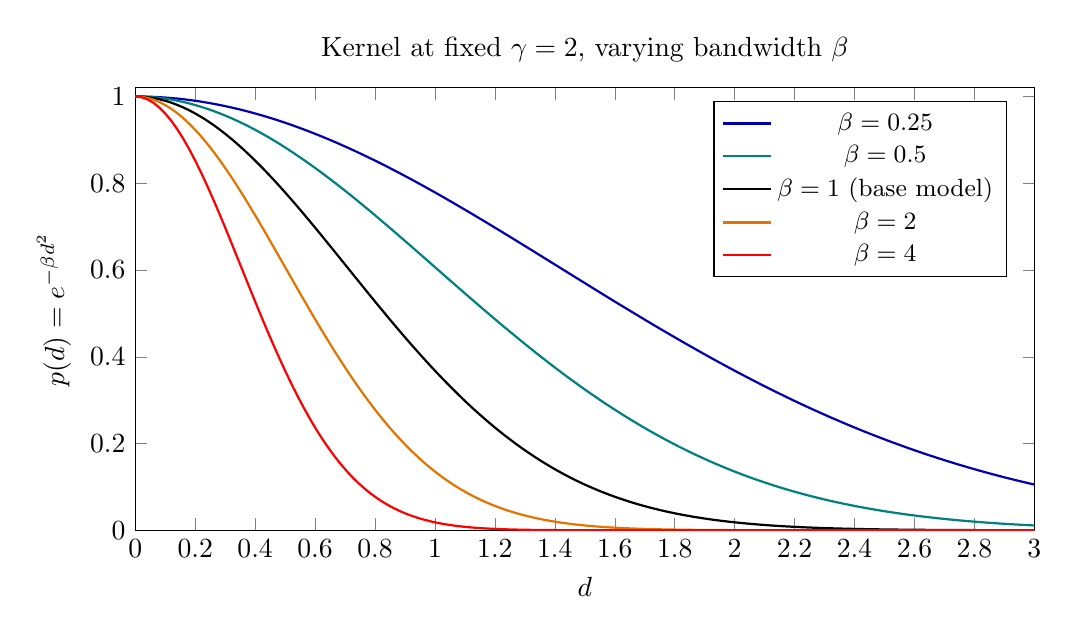
\begin{tikzpicture}
\begin{axis}[
  width=13cm,height=7.2cm,
  xlabel={$d$}, ylabel={$p(d)=e^{-\bw d^{2}}$},
  xmin=0,xmax=3, ymin=0, ymax=1.02,
  domain=0:3, samples=150,
  legend pos=north east,
  title={Kernel at fixed $\gamma=2$, varying bandwidth $\bw$},
  legend style={font=\small},
]
\addplot[thick,blue!70!black]        {exp(-0.25*x^2)}; \addlegendentry{$\bw=0.25$}
\addplot[thick,teal]                 {exp(-0.5*x^2)};  \addlegendentry{$\bw=0.5$}
\addplot[thick,black]                {exp(-1*x^2)};    \addlegendentry{$\bw=1$ (base model)}
\addplot[thick,orange!90!black]      {exp(-2*x^2)};    \addlegendentry{$\bw=2$}
\addplot[thick,red]                  {exp(-4*x^2)};    \addlegendentry{$\bw=4$}
\end{axis}
\end{tikzpicture}
\caption{Increasing the bandwidth $\bw$ narrows the kernel: a cell feels a
target only if it is much closer, for the same exponent $\gamma$.}
\label{fig:kernel_beta}
\end{figure}

\begin{figure}[H]
\centering
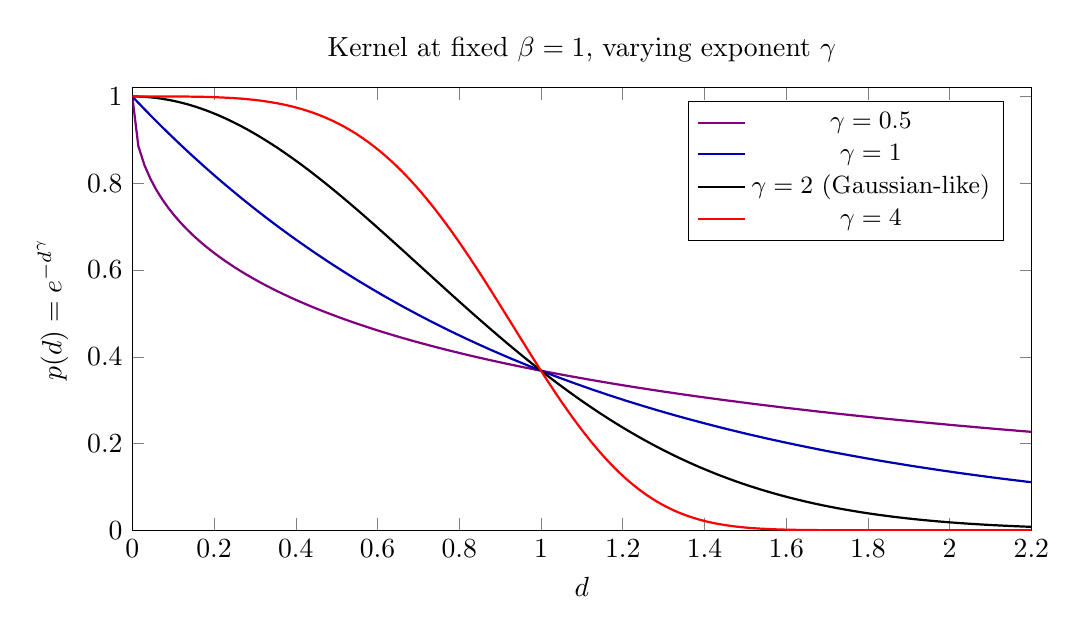
\begin{tikzpicture}
\begin{axis}[
  width=13cm,height=7.2cm,
  xlabel={$d$}, ylabel={$p(d)=e^{-d^{\gamma}}$},
  xmin=0,xmax=2.2, ymin=0, ymax=1.02,
  domain=0:2.2, samples=150,
  legend pos=north east,
  title={Kernel at fixed $\bw=1$, varying exponent $\gamma$},
  legend style={font=\small},
]
\addplot[thick,violet]          {exp(-x^0.5)}; \addlegendentry{$\gamma=0.5$}
\addplot[thick,blue!70!black]   {exp(-x^1)};   \addlegendentry{$\gamma=1$}
\addplot[thick,black]           {exp(-x^2)};   \addlegendentry{$\gamma=2$ (Gaussian-like)}
\addplot[thick,red]             {exp(-x^4)};   \addlegendentry{$\gamma=4$}
\end{axis}
\end{tikzpicture}
\caption{The exponent $\gamma$ changes the \emph{shape} of the decay, not
just its scale: large $\gamma$ produces an almost flat plateau followed by a
sharp cliff.}
\label{fig:kernel_gamma}
\end{figure}

Because $\gamma$ and $\bw$ enter the kernel jointly, the effect of increasing
$\gamma$ is not the same at every bandwidth. Figure~\ref{fig:kernel_gamma_by_beta}
repeats the $\gamma$-sweep of Figure~\ref{fig:kernel_gamma} at three
bandwidths — broad ($\bw=0.5$), the base model ($\bw=1$), and narrow
($\bw=2$) — side by side.

\begin{figure}[H]
\centering
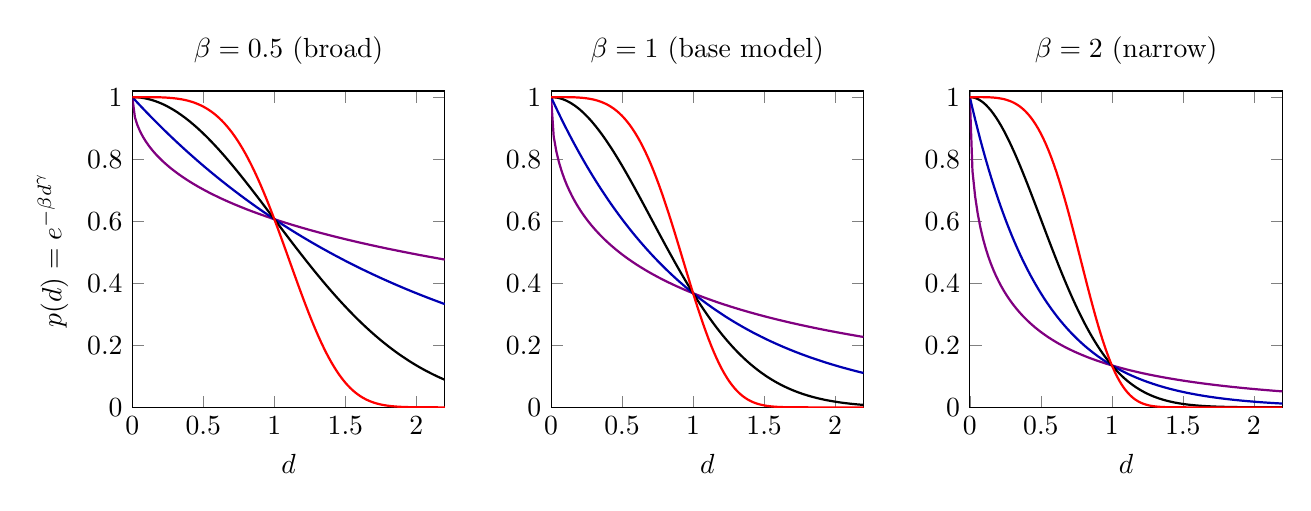
\begin{tikzpicture}
\begin{groupplot}[
  group style={group size=3 by 1, horizontal sep=1.35cm},
  width=5.55cm, height=5.6cm,
  domain=0:2.2, samples=120,
  xlabel={$d$},
  xmin=0,xmax=2.2, ymin=0, ymax=1.02,
  legend columns=4,
  legend to name=kernelgammalegend,
  legend style={font=\small},
]
\nextgroupplot[title={$\bw=0.5$ (broad)}, ylabel={$p(d)=e^{-\bw d^{\gamma}}$}]
\addplot[thick,violet]        {exp(-0.5*x^0.5)}; \addlegendentry{$\gamma=0.5$}
\addplot[thick,blue!70!black] {exp(-0.5*x^1)};   \addlegendentry{$\gamma=1$}
\addplot[thick,black]         {exp(-0.5*x^2)};   \addlegendentry{$\gamma=2$}
\addplot[thick,red]           {exp(-0.5*x^4)};   \addlegendentry{$\gamma=4$}

\nextgroupplot[title={$\bw=1$ (base model)}]
\addplot[thick,violet]        {exp(-x^0.5)};
\addplot[thick,blue!70!black] {exp(-x^1)};
\addplot[thick,black]         {exp(-x^2)};
\addplot[thick,red]           {exp(-x^4)};

\nextgroupplot[title={$\bw=2$ (narrow)}]
\addplot[thick,violet]        {exp(-2*x^0.5)};
\addplot[thick,blue!70!black] {exp(-2*x^1)};
\addplot[thick,black]         {exp(-2*x^2)};
\addplot[thick,red]           {exp(-2*x^4)};
\end{groupplot}
\end{tikzpicture}

\vspace{2mm}
\centering\ref{kernelgammalegend}
\caption{The effect of increasing $\gamma$ under three bandwidth regimes. In
every panel, larger $\gamma$ still produces the same qualitative
transition — from a cusped, heavy-shouldered profile toward a flat plateau
with a sharp cliff — but a broad kernel ($\bw<1$, left) keeps that cliff
pushed out to larger $d$, while a narrow kernel ($\bw>1$, right) pulls the
entire family in toward the origin. Shape ($\gamma$) and scale ($\bw$)
therefore act on the kernel independently, but their visible effect on any
one curve is not: the same $\gamma$ reads as a very different kernel width
depending on $\bw$.}
\label{fig:kernel_gamma_by_beta}
\end{figure}

\begin{keybox}[Reading the two knobs together]
$\gamma$ sets the \emph{shape} of the interaction (how abruptly it turns
off); $\bw$ sets the \emph{scale} at which that shape is applied. As shown
below, this separation of roles is exactly what allows $\bw$ to shift the
location and even the character of the bifurcation without altering the
underlying exponent $\gamma$.
\end{keybox}

% ============================================================
\section{The collective flow with bandwidth}
\label{sec:model}
% ============================================================

The population objective is unchanged in form:
\[
  F(\bx_1,\ldots,\bx_N)=\prod_{i=1}^{k}S_i,
  \qquad
  S_i=\sum_{j=1}^{N}p_{ij},
  \qquad
  p_{ij}=e^{-\bw d_{ij}^{\gamma}},
  \qquad
  d_{ij}=\norm{\bx_j-\ba_i}.
\]
Hence
\[
  \log F=\sum_{i=1}^{k}\log S_i,
  \qquad
  \dot{\bx}_j=\nabla_{\bx_j}\log F=\sum_{i=1}^{k}\frac{1}{S_i}\nabla_{\bx_j}p_{ij},
\]
where the second equality uses $\partial S_i/\partial\bx_j=\partial
p_{ij}/\partial \bx_j$ (only the $j$-th summand of $S_i$ depends on $\bx_j$).

\subsection{Gradient of the kernel}

Write $\br_{ij}=\bx_j-\ba_i$. Since $\nabla d=\br/d$,
\[
  \nabla d^{\gamma}=\gamma d^{\gamma-1}\nabla d=\gamma d^{\gamma-2}\br,
\]
which is unchanged by the bandwidth (it is purely a property of the distance
function). Therefore
\begin{align}
  \nabla_{\bx_j}p_{ij}
  &=
  \nabla_{\bx_j}\exp\!\big(-\bw d_{ij}^{\gamma}\big)
  \nonumber\\
  &=
  -\bw\,\big(\nabla d_{ij}^{\gamma}\big)\,e^{-\bw d_{ij}^{\gamma}}
  \nonumber\\
  &=
  -\bw\gamma\, d_{ij}^{\gamma-2}\,p_{ij}\,\br_{ij}.
  \label{eq:grad_p_beta}
\end{align}

\subsection{The exact flow}

Substituting \eqref{eq:grad_p_beta} into $\dot{\bx}_j$:
\begin{equation}
  \boxed{
  \dot{\bx}_j
  =
  -\bw\gamma
  \sum_{i=1}^{k}
  \frac{p_{ij}}{S_i}
  d_{ij}^{\gamma-2}
  (\bx_j-\ba_i).
  }
  \label{eq:exact_gradient_beta}
\end{equation}
This is identical in form to the base-model flow, with the single
replacement $\gamma\mapsto\bw\gamma$ in the \emph{overall prefactor} — but,
as the next sections show, $\bw$ also enters \emph{inside} every stability
eigenvalue, not merely as an overall rate.

\subsection{The single-cell limit: performance as a product across tasks}
\label{sec:single_cell}

It is worth pausing on the special case $N=1$ before returning to the
population, since it is what actually justifies the multiplicative form of
$F$ in the first place.

\begin{definition}[Performance on a task]
The performance of a cell at position $\bx$ on task (target) $i$ is the
kernel value itself,
\begin{equation}
  \boxed{
  \pi_i(\bx):=e^{-\bw d_i^{\gamma}},
  \qquad d_i=\norm{\bx-\ba_i}.
  }
  \label{eq:performance_def}
\end{equation}
It equals $1$ exactly at the archetype $\ba_i$ and decays toward $0$ as the
cell moves away, at the rate set by $(\bw,\gamma)$ studied in
Section~\ref{sec:kernel}.
\end{definition}

\begin{proposition}[Single-cell objective is a product of task performances]
\label{prop:single_cell_product}
Let $m$ denote the number of tasks (this is the quantity called $k$
elsewhere in this document). For $N=1$,
\begin{equation}
  \boxed{
  F(\bx)\Big|_{N=1}=\prod_{i=1}^{m}\pi_i(\bx).
  }
  \label{eq:single_cell_product}
\end{equation}
\end{proposition}
\begin{proof}
With a single cell, every per-task sum has exactly one summand:
\[
  S_i=\sum_{j=1}^{N}p_{ij}\bigg|_{N=1}=p_{i1}=e^{-\bw d_{i1}^{\gamma}}=\pi_i(\bx).
\]
Since $F=\prod_{i=1}^m S_i$ by definition (Section~\ref{sec:model}),
substituting gives $F|_{N=1}=\prod_{i=1}^m\pi_i(\bx)$ directly.
\end{proof}

\begin{remark}
Proposition~\ref{prop:single_cell_product} shows that the population-level
rule — multiply the per-task totals $S_i$ across tasks — is exactly the
$N$-cell generalization of the more primitive, single-organism statement
that overall fitness is the \emph{product}, not the sum, of task
performances. $S_i$ plays, for the population, precisely the role that
$\pi_i$ plays for the individual cell: it is the total performance
delivered on task $i$, still combined multiplicatively across tasks.
\end{remark}

\begin{corollary}[Multiplicative performance is additive cost]
\label{cor:additive_cost}
Taking logarithms of \eqref{eq:single_cell_product},
\begin{equation}
  \boxed{
  \log F(\bx)\Big|_{N=1}=\sum_{i=1}^{m}\log\pi_i(\bx)=-\bw\sum_{i=1}^{m}d_i^{\gamma}.
  }
  \label{eq:additive_cost}
\end{equation}
Hence maximizing the multiplicative performance $\prod_i\pi_i(\bx)$ is
exactly equivalent to minimizing the additive, $\gamma$-weighted total cost
$C(\bx)=\bw\sum_{i=1}^m d_i^{\gamma}$: multiplicative performance and
additive cost are the same object viewed on two different scales.
\end{corollary}

\begin{warningbox}[Why a product, not a sum, of performances]
The product structure encodes an \emph{AND} across tasks rather than an
\emph{OR}. If a cell fails one task entirely, $\pi_i\to0$, then
$F=\prod_i\pi_i\to0$ regardless of how well it performs on every other
task — one weak link collapses total fitness. An additive combination
$\sum_i\pi_i$ would instead let excellence on one task compensate for
failure on another. It is this all-or-nothing requirement — good at
\emph{every} task simultaneously, not merely on average — that gives the
model its Pareto character, and it is ultimately what forces a
\emph{population} to specialize (Sections~\ref{sec:transverse}--\ref{sec:classification})
rather than settle everyone at a single shared compromise.
\end{warningbox}

\begin{proposition}[Single-cell dynamics]
\label{prop:single_cell_dynamics}
The gradient flow of an isolated cell is
\begin{equation}
  \boxed{
  \dot{\bx}=\nabla\log F(\bx)\Big|_{N=1}=-\bw\gamma\sum_{i=1}^{m}d_i^{\gamma-2}(\bx-\ba_i).
  }
  \label{eq:single_cell_flow}
\end{equation}
\end{proposition}
\begin{proof}
Set $N=1$ in \eqref{eq:exact_gradient_beta}. With a single cell, $S_i=p_{i1}$
exactly, so the ratio appearing there is identically
\[
  \frac{p_{i1}}{S_i}=\frac{p_{i1}}{p_{i1}}=1
\]
for the (only) cell $j=1$. Substituting into \eqref{eq:exact_gradient_beta}
gives \eqref{eq:single_cell_flow} directly. Equivalently, this is just
$\dot{\bx}=-\nabla C(\bx)$ for the cost of Corollary~\ref{cor:additive_cost}.
\end{proof}

\begin{proposition}[Single-cell stability tensor]
\label{prop:single_cell_stability}
Let $J^{(1)}(\bx)=D_{\bx}\dot{\bx}=\nabla^2\log F(\bx)\big|_{N=1}$ be the
Jacobian of the single-cell flow \eqref{eq:single_cell_flow} at any point
$\bx$ (not necessarily an equilibrium) — i.e.\ the ordinary $D\times D$
matrix of partial derivatives of the vector field $\dot{\bx}=f(\bx)$ on
$\R^D$ ($D=2$ in the planar examples below). This is the same word used for
the collective Jacobian $J_{jk}$ of
Section~\ref{sec:transverse}, but a much simpler object: there is only one
cell, so there are no cell indices $j,k$ to couple, and $J^{(1)}$ is
literally the Hessian of $\log F$ rather than a block matrix built from it.
Then
\begin{equation}
  \boxed{
  J^{(1)}(\bx)=-\bw\gamma\sum_{i=1}^{m}d_i^{\gamma-2}\Big[I+(\gamma-2)\hat\br_i\hat\br_i^{\top}\Big],
  }
  \label{eq:single_cell_jacobian}
\end{equation}
and for a unit direction $\be$, the directional eigenvalue is
\begin{equation}
  \boxed{
  \lambda^{(1)}(\be;\bx)=\be^{\top}J^{(1)}(\bx)\be
  =
  -\bw\gamma\sum_{i=1}^{m}d_i^{\gamma-2}\Big[1+(\gamma-2)(\be\cdot\hat\br_i)^2\Big].
  }
  \label{eq:single_cell_eigenvalue}
\end{equation}
At any equilibrium $\bx^*$ of \eqref{eq:single_cell_flow}, $\bx^*$ is locally
stable in direction $\be$ iff $\lambda^{(1)}(\be;\bx^*)<0$, and unstable iff
$\lambda^{(1)}(\be;\bx^*)>0$, by the usual linearization
$\dot{\delta\bx}=J^{(1)}(\bx^*)\delta\bx$.
\end{proposition}
\begin{proof}
Differentiate \eqref{eq:single_cell_flow} once more. Writing
$g_i(\bx)=d_i^{\gamma-2}\br_i$ (so that $\dot{\bx}=-\bw\gamma\sum_ig_i$), the
product rule gives
\[
  \nabla g_i
  =
  \big(\nabla d_i^{\gamma-2}\big)\br_i^{\top}+d_i^{\gamma-2}\nabla\br_i
  =
  (\gamma-2)d_i^{\gamma-4}\br_i\br_i^{\top}+d_i^{\gamma-2}I,
\]
using $\nabla d_i^{\gamma-2}=(\gamma-2)d_i^{\gamma-4}\br_i$ (the same
identity as $\nabla d^{\gamma}=\gamma d^{\gamma-2}\br$, with exponent
$\gamma-2$ in place of $\gamma$) and $\nabla\br_i=I$. Since
$\br_i\br_i^{\top}=d_i^2\hat\br_i\hat\br_i^{\top}$,
\[
  \nabla g_i=d_i^{\gamma-2}\Big[I+(\gamma-2)\hat\br_i\hat\br_i^{\top}\Big],
\]
and summing with the prefactor $-\bw\gamma$ gives
\eqref{eq:single_cell_jacobian}. Equation~\eqref{eq:single_cell_eigenvalue}
follows by contracting with $\be$ on both sides.
\end{proof}

\begin{remark}[A structurally simpler eigenvalue than the collective case]
Compare \eqref{eq:single_cell_eigenvalue} with the collective directional
eigenvalue \eqref{eq:lambda_dir_beta}. The collective formula contains the
term $\bw\gamma d_i^{\gamma}$ \emph{inside} the bracket — this is exactly
what let $\bw$ shift the location of the bifurcation in
Sections~\ref{sec:critical_bandwidth}--\ref{sec:classification}. The
single-cell formula \eqref{eq:single_cell_eigenvalue} has no such term: the
bracket $\big[1+(\gamma-2)(\be\cdot\hat\br_i)^2\big]$ depends only on
$\gamma$ and geometry, never on $\bw$. This is a direct consequence of
$\log$ undoing the kernel's exponential for a single cell (Corollary
\ref{cor:additive_cost}): the population's normalizing sum $S_i$ is what
reintroduces the nonlinear $\bw\gamma d_i^{\gamma}$ dependence into the
collective eigenvalue, and a lone cell has no such sum. Concretely, this
means bandwidth can rescale the \emph{rate} of a single cell's stability or
instability, but — unlike in the population — it can never flip its
\emph{sign}. Section~\ref{sec:two_transverse} makes this precise on the
two-target axis.
\end{remark}

\begin{remark}[Specialization is a collective phenomenon]
Unlike the $N$-cell flow \eqref{eq:exact_gradient_beta}, the single-cell
flow \eqref{eq:single_cell_flow} has no normalizing denominator at all:
there is no other cell to share task coverage with, so the entire
competitive mechanism that later produces \emph{population} symmetry
breaking (Sections~\ref{sec:transverse}--\ref{sec:classification}) is
simply absent. This does not mean a single cell's own trajectory is always
stable, however — Proposition~\ref{prop:single_cell_stability} shows it has
genuine transverse eigenvalues of its own, and Section~\ref{sec:two_transverse}
finds a regime where they are positive. What is absent for $N=1$ is
specifically the mechanism by which a \emph{population} splits into
distinct sub-groups; an unstable single cell simply drifts off its
symmetric path toward one target, which is not yet ``specialization'' in
the collective sense, only the loss of a symmetric trajectory. For $m\ge2$
distinct targets, an isolated cell instead settles — when it settles — at a
single compromise point minimizing $C(\bx)=\bw\sum_id_i^\gamma$ across all
targets simultaneously.
\end{remark}

% ============================================================
\section{Two symmetric targets: axial motion}
\label{sec:two_axis}
% ============================================================

Take $\ba_1=(-1,0)$, $\ba_2=(1,0)$ and a source on the symmetry axis,
$\bx_j(t)=(0,y(t))$ for every $j$. Both targets are equidistant:
\[
  d(y)=\sqrt{1+y^2}.
\]
On the axis, $S_1=S_2=Ne^{-\bw d^{\gamma}}$, so
\[
  \log F = 2\log N - 2\bw d^{\gamma}.
\]
Differentiating with respect to $y$ and dividing by $N$ (each of the $N$
cells contributes the same axial pull, and $S_i$ already carries the factor
of $N$):
\begin{equation}
  \boxed{
  \dot y = -\kappa(y)\,y,
  \qquad
  \kappa(y)=\frac{2\bw\gamma}{N}(1+y^2)^{(\gamma-2)/2}>0.
  }
  \label{eq:ydot_beta}
\end{equation}
Near $y=0$, $\dot y\approx-\dfrac{2\bw\gamma}{N}y$, so
\[
  y(t)\sim y_0\, e^{-2\bw\gamma t/N}.
\]
The axial approach to the symmetric terminal point is therefore still
monotone and asymptotic for any $\bw>0$; increasing $\bw$ (or $\gamma$)
simply speeds up this approach along the axis. This part of the picture is
qualitatively unchanged from the base model — the interesting effect of
$\bw$ appears entirely in the \emph{transverse} direction.

% ============================================================
\section{Transverse stability: full re-derivation}
\label{sec:transverse}
% ============================================================

\subsection{Hessian of the bandwidth-modified kernel}

Let $\phi=\bw d^{\gamma}$, so $p=e^{-\phi}$. Using the standard identity
$\nabla^2 e^{-\phi}=e^{-\phi}\big[(\nabla\phi)(\nabla\phi)^{\top}-\nabla^2\phi\big]$,
we need $\nabla\phi$ and $\nabla^2\phi$.

Since $\nabla d^\gamma=\gamma d^{\gamma-2}\br$,
\[
  \nabla\phi=\bw\gamma d^{\gamma-2}\br.
\]
For the Hessian of $d^\gamma$ itself (unchanged from the base model's
Appendix~A, since it does not involve $\bw$):
\[
  \nabla^2 d^{\gamma}
  =
  \gamma\Big[d^{\gamma-2}I+(\gamma-2)d^{\gamma-4}\br\br^{\top}\Big],
\]
so
\[
  \nabla^2\phi=\bw\gamma\Big[d^{\gamma-2}I+(\gamma-2)d^{\gamma-4}\br\br^{\top}\Big].
\]
Also
\[
  (\nabla\phi)(\nabla\phi)^{\top}=\bw^2\gamma^2 d^{2\gamma-4}\br\br^{\top}.
\]
Combining,
\begin{align}
  \nabla^2 p
  &=
  e^{-\phi}
  \Big[
    \bw^2\gamma^2 d^{2\gamma-4}\br\br^{\top}
    -
    \bw\gamma d^{\gamma-2}I
    -
    \bw\gamma(\gamma-2)d^{\gamma-4}\br\br^{\top}
  \Big]
  \nonumber\\[4pt]
  &=
  \boxed{
  \bw\gamma\, e^{-\bw d^{\gamma}}\, d^{\gamma-4}
  \Big[
    \big(\bw\gamma d^{\gamma}-(\gamma-2)\big)\,\br\br^{\top}
    -
    d^2 I
  \Big].
  }
  \label{eq:hessian_kernel_beta}
\end{align}
At $\bw=1$ this reduces exactly to the base model's kernel Hessian.

\subsection{The collective transverse operator}

Consider $N$ co-located cells at a common point $\bx$, with $k$ targets
$\ba_i$, $d_i=\norm{\bx-\ba_i}$, $\hat\br_i=(\bx-\ba_i)/d_i$. At this
configuration $S_i=N p_i(\bx)$.

Writing the flow as $\dot{\bx}_j=\sum_i g_i(\bx_j)/S_i$ with
$g_i=\nabla p_i$, and linearising about the co-located point, the Jacobian
block coupling cells $j$ and $k$ is
\[
  J_{jk}
  =
  H\,\delta_{jk}-Q,
  \qquad
  H=\sum_i\frac{\nabla^2 p_i}{S_i}=\frac{1}{N}\sum_i\frac{\nabla^2 p_i}{p_i},
  \qquad
  Q=\sum_i\frac{(\nabla p_i)(\nabla p_i)^{\top}}{S_i^2}.
\]
For a \emph{zero-sum} perturbation $\sum_j\delta\bx_j=0$ (the population's
internal, symmetry-breaking modes), the $Q$-term cancels identically:
\[
  (J\,\delta\bx)_j=H\delta\bx_j-Q\sum_k\delta\bx_k=H\delta\bx_j.
\]
So the transverse stability operator is simply $H$. Using
\eqref{eq:hessian_kernel_beta} with $\br_i\br_i^{\top}=d_i^2\hat\br_i\hat\br_i^{\top}$,
\begin{equation}
  H
  =
  \frac{\bw\gamma}{N}
  \sum_i d_i^{\gamma-2}
  \Big[
    \big(\bw\gamma d_i^{\gamma}-\gamma+2\big)\hat\br_i\hat\br_i^{\top}-I
  \Big]
  \;=\;
  M(\bx)-\tau(\bx)I
  \;\equiv\;\Lsplit(\bx),
  \label{eq:H_split}
\end{equation}
with
\begin{equation}
  \boxed{
  M(\bx)=\frac{\bw\gamma}{N}\sum_i d_i^{\gamma-2}\big(\bw\gamma d_i^{\gamma}-\gamma+2\big)\hat\br_i\hat\br_i^{\top},
  \qquad
  \tau(\bx)=\frac{\bw\gamma}{N}\sum_i d_i^{\gamma-2}.
  }
  \label{eq:M_tau_beta}
\end{equation}
For a unit direction $\be$, the directional eigenvalue is
\begin{equation}
  \boxed{
  \lambda(\be)=\be^{\top}\Lsplit\be
  =
  \frac{\bw\gamma}{N}\sum_i d_i^{\gamma-2}
  \Big[
    \big(\bw\gamma d_i^{\gamma}-\gamma+2\big)(\be\cdot\hat\br_i)^2-1
  \Big].
  }
  \label{eq:lambda_dir_beta}
\end{equation}
Equations \eqref{eq:M_tau_beta}--\eqref{eq:lambda_dir_beta} generalize the
base model's Appendix~B and C by the single, uniform replacement
$\gamma d_i^{\gamma}\mapsto\bw\gamma d_i^{\gamma}$ inside every bracket, with
an overall prefactor $\gamma\mapsto\bw\gamma$. Every other factor
($d_i^{\gamma-2}$, the $-\gamma+2$ term, the $-1$) is untouched, because
those come from the geometric Hessian of $d^\gamma$, not from the kernel's
overall scale.

% ============================================================
\section{The two-target transverse eigenvalue}
\label{sec:two_transverse}
% ============================================================

For $\ba_{1,2}=(\mp1,0)$ and $\bx=(0,y)$, both targets share $d=\sqrt{1+y^2}$
and $(\be_x\cdot\hat\br_{1,2})^2=1/d^2$. Equation~\eqref{eq:lambda_dir_beta}
with $\be=\be_x$ gives, after doubling for the two identical targets,
\[
  \lsplit
  =
  \frac{2\bw\gamma}{N}d^{\gamma-2}
  \left[\frac{\bw\gamma d^\gamma-\gamma+2}{d^2}-1\right]
  =
  \frac{2\bw\gamma}{N}d^{\gamma-4}\big[\bw\gamma d^{\gamma}-\gamma+2-d^2\big].
\]
Introduce $u=d^2=1+y^2$ and define
\begin{equation}
  \boxed{
  \phib(u)=\bw\gamma\,u^{\gamma/2}-u-(\gamma-2).
  }
  \label{eq:phi_beta}
\end{equation}
Then
\begin{equation}
  \boxed{
  \lsplit(y)=\frac{2\bw\gamma}{N}(1+y^2)^{(\gamma-4)/2}\,\phib\big(1+y^2\big).
  }
  \label{eq:lsplit_beta}
\end{equation}
Since the prefactor $\frac{2\bw\gamma}{N}(1+y^2)^{(\gamma-4)/2}$ is strictly
positive for all $\bw,\gamma>0$ and all $y$,
\begin{equation}
  \boxed{
  \operatorname{sign}\big(\lsplit(y)\big)=\operatorname{sign}\big(\phib(1+y^2)\big).
  }
  \label{eq:sign_correspondence}
\end{equation}
This single fact is the key to everything that follows: the entire
transverse-stability question reduces to the sign of the scalar function
$\phib(u)$ on $u\ge1$.

\subsection{The single-cell version, and why it is different}
\label{sec:two_transverse_single}

It is instructive to run the identical computation for a single cell
($N=1$) on the same axis, using
Proposition~\ref{prop:single_cell_stability} in place of the collective
tensor. With $\be=\be_x$ and $(\be_x\cdot\hat\br_{1,2})^2=1/d^2$,
\eqref{eq:single_cell_eigenvalue} gives, after doubling for the two
identical targets,
\begin{equation}
  \lambda_x^{(1)}(y)
  =
  -2\bw\gamma\,d^{\gamma-2}\left[1+\frac{\gamma-2}{d^2}\right]
  =
  -2\bw\gamma\,d^{\gamma-4}\big[d^2+\gamma-2\big].
  \label{eq:single_cell_lambda_x}
\end{equation}
With $u=d^2=1+y^2$ as before, define
\begin{equation}
  \boxed{
  \psi(u)=u+(\gamma-2),
  }
  \label{eq:psi_single}
\end{equation}
so that
\begin{equation}
  \boxed{
  \lambda_x^{(1)}(y)=-2\bw\gamma\,(1+y^2)^{(\gamma-4)/2}\,\psi\big(1+y^2\big).
  }
  \label{eq:lambda_x_single}
\end{equation}
The prefactor $-2\bw\gamma(1+y^2)^{(\gamma-4)/2}$ is strictly \emph{negative}
for all $\bw,\gamma>0$, so
\begin{equation}
  \boxed{
  \operatorname{sign}\big(\lambda_x^{(1)}(y)\big)=-\operatorname{sign}\big(\psi(1+y^2)\big).
  }
  \label{eq:sign_correspondence_single}
\end{equation}

\begin{proposition}[Single-cell terminal stability and critical height]
\label{prop:single_cell_critical}
On the two-target axis, the single-cell terminal point ($y=0$) satisfies
\begin{equation}
  \boxed{
  \lambda_x^{(1)}(0)=-2\bw\gamma(\gamma-1).
  }
  \label{eq:lambda_x_terminal_single}
\end{equation}
Consequently:
\begin{itemize}[leftmargin=1.4em]
\item if $\gamma>1$: $\lambda_x^{(1)}(y)<0$ for every $y$ — the single
      cell's symmetric trajectory is transversely stable everywhere;
\item if $\gamma=1$: $\lambda_x^{(1)}(y)=0$ at $y=0$ and $\lambda_x^{(1)}(y)<0$
      for $y\ne0$ — exactly marginal at the terminal point;
\item if $\gamma<1$: $\lambda_x^{(1)}(y)>0$ for $|y|<y_c^{(1)}$ and
      $\lambda_x^{(1)}(y)<0$ for $|y|>y_c^{(1)}$, with critical height
      \begin{equation}
        \boxed{y_c^{(1)}(\gamma)=\sqrt{1-\gamma}.}
        \label{eq:yc_single}
      \end{equation}
\end{itemize}
\end{proposition}
\begin{proof}
Since $\psi$ is affine in $u$ (unlike $\phib$, it is neither concave nor
convex — it is exactly linear), its sign on $u\ge1$ is settled directly:
$\psi(u)\ge0 \iff u\ge2-\gamma$. If $\gamma\ge1$ then $2-\gamma\le1\le u$
always, so $\psi(u)\ge0$ throughout, with equality only possible at
$u=1,\gamma=1$; by \eqref{eq:sign_correspondence_single} this gives
$\lambda_x^{(1)}\le0$ throughout, i.e.\ the first two bullets. If
$\gamma<1$ then $2-\gamma>1$, so $\psi(u)<0$ exactly on
$1\le u<2-\gamma$, i.e.\ $y^2<1-\gamma$, giving $\lambda_x^{(1)}>0$ there by
\eqref{eq:sign_correspondence_single}; solving $u=2-\gamma$ for $y$ gives
$y_c^{(1)}=\sqrt{1-\gamma}$ exactly.
\end{proof}

\begin{warningbox}[Single-cell instability is real, but structurally
different from the collective one]
For $\gamma<1$, a lone cell placed exactly on the axis within
$|y|<\sqrt{1-\gamma}$ of the terminal point will, under any lateral
perturbation, drift away from the axis toward one target rather than
converge to the shared point — its own trajectory is transversely
unstable, with no population involved at all. But compare
\eqref{eq:psi_single} with $\phib$ in \eqref{eq:phi_beta}: the single-cell
function $\psi(u)=u+(\gamma-2)$ contains no $\bw$ whatsoever, while
$\phib(u)=\bw\gamma u^{\gamma/2}-u-(\gamma-2)$ does. Bandwidth therefore
changes \emph{how fast} the single cell's instability grows (through the
overall prefactor $\bw\gamma$) but can never change \emph{whether} it
occurs, nor where $y_c^{(1)}$ sits — that depends on $\gamma$ alone. The
critical bandwidth $\bwc(\gamma)$ of Section~\ref{sec:critical_bandwidth} is
a genuinely collective effect, made possible only because the population's
normalizing sum $S_i$ reintroduces $\bw\gamma d_i^\gamma$ into the
eigenvalue — exactly the term a single cell's $\log$ cancels away
(Corollary~\ref{cor:additive_cost}).
\end{warningbox}

\begin{center}
\renewcommand{\arraystretch}{1.3}
\begin{tabular}{@{}lll@{}}
\toprule
& \textbf{Single cell ($N=1$)} & \textbf{Population ($N$-cell)} \\
\midrule
Stability function & $\psi(u)=u+(\gamma-2)$, linear & $\phib(u)=\bw\gamma u^{\gamma/2}-u-(\gamma-2)$ \\
Depends on $\bw$? & no (prefactor only) & yes, inside the bracket \\
Terminal threshold & $\gamma=1$ & $\bw=\bwc(\gamma)=1-1/\gamma$ (for $\gamma>1$) \\
Unstable region & $\gamma<1$, $|y|<\sqrt{1-\gamma}$ & $\bw>\bwc(\gamma)$ (or the inverted case, Sec.~\ref{sec:classification}) \\
\bottomrule
\end{tabular}
\end{center}

\subsection{The concrete global picture: what actually happens for $\gamma<1$ versus $\gamma>1$}
\label{sec:single_cell_global}

Proposition~\ref{prop:single_cell_critical} is a \emph{local} statement: it
only says whether the symmetric point is stable to infinitesimal
perturbations. It does not say whether that local behavior is the whole
story globally, nor where an unstable trajectory actually ends up. Both
questions have complete, concrete answers.

\begin{lemma}[Convexity of the single-cell cost for $\gamma\ge1$]
\label{lem:cost_convex}
For $\gamma\ge1$ and any targets $\ba_1,\ldots,\ba_m\in\R^D$, the cost
\begin{equation}
  \boxed{
  C(\bx)=\bw\sum_{i=1}^{m}\norm{\bx-\ba_i}^{\gamma}
  }
  \label{eq:cost_def}
\end{equation}
is convex on $\R^D$, and coercive: $C(\bx)\to\infty$ as $\norm{\bx}\to\infty$.
\end{lemma}
\begin{proof}
The scalar map $t\mapsto t^{\gamma}$ is convex and nondecreasing on
$[0,\infty)$ for $\gamma\ge1$, since $\frac{d}{dt}t^\gamma=\gamma
t^{\gamma-1}\ge0$ and $\frac{d^2}{dt^2}t^\gamma=\gamma(\gamma-1)t^{\gamma-2}\ge0$.
The map $\bx\mapsto\norm{\bx-\ba_i}$ is convex (a norm composed with a
translation). The composition of a convex, nondecreasing scalar function
with a convex function is convex, so each $\norm{\bx-\ba_i}^\gamma$ is
convex; $C$, a nonnegative sum of such terms, is therefore convex.
Coercivity is immediate, since each individual summand already tends to
$\infty$ as $\norm{\bx}\to\infty$.
\end{proof}

\begin{theorem}[Global convergence for $\gamma\ge1$]
\label{thm:global_convergence}
For $\gamma\ge1$, the single-cell flow \eqref{eq:single_cell_flow} (which is
exactly $\dot{\bx}=-\nabla C(\bx)$ for the cost \eqref{eq:cost_def}, by
Corollary~\ref{cor:additive_cost}) converges, from \emph{every} initial
condition, to the set of global minimizers of $C$. On the two-target axis
this set is
\begin{equation}
  \boxed{
  \arg\min C=
  \begin{cases}
  \{(0,0)\} & \gamma>1,\\[2pt]
  \{(x,0):-1\le x\le1\} & \gamma=1.
  \end{cases}
  }
  \label{eq:argmin_two_target}
\end{equation}
\end{theorem}
\begin{proof}
Along any trajectory of $\dot{\bx}=-\nabla C(\bx)$,
\[
  \frac{d}{dt}C(\bx(t))=\nabla C(\bx(t))\cdot\dot{\bx}(t)=-\norm{\nabla C(\bx(t))}^2\le0,
\]
with equality iff $\bx(t)$ is a critical point of $C$. So $C$ decreases
strictly along the flow except at critical points. By
Lemma~\ref{lem:cost_convex}, $C$ is coercive, so every sublevel set
$\{C\le c\}$ is closed and bounded, hence compact, and the trajectory
remains in one such set for all $t\ge0$. LaSalle's invariance principle
then gives convergence to the largest invariant subset of
$\{\nabla C=0\}$, i.e.\ to the critical-point set of $C$. Since $C$ is
convex, every critical point is a global minimizer, proving the first
claim. On the connecting segment $\Sigma=\{(x,0):-1<x<1\}$, where
$C(x,0)=\bw[(x+1)^\gamma+(1-x)^\gamma]$,
\[
  C'(x)=\bw\gamma\big[(x+1)^{\gamma-1}-(1-x)^{\gamma-1}\big],
\]
which vanishes iff $(x+1)^{\gamma-1}=(1-x)^{\gamma-1}$. For $\gamma>1$ the
map $t\mapsto t^{\gamma-1}$ is injective on $(0,\infty)$, forcing $x+1=1-x$,
i.e.\ $x=0$ uniquely; for $\gamma=1$ both sides equal $1$ identically, so
every $x\in(-1,1)$ is a critical point. Off $\Sigma$, the two-target
reflection symmetry leaves $(0,0)$ as the only point where $\nabla C=0$ can
hold in the transverse direction as well (Proposition~\ref{prop:single_cell_critical}
already verifies this is a critical point for every $\gamma$), giving
\eqref{eq:argmin_two_target}.
\end{proof}

\begin{warningbox}[This upgrades a local result to a global one]
For $\gamma>1$, Proposition~\ref{prop:single_cell_critical} only established
that $(0,0)$ is \emph{locally} stable. Theorem~\ref{thm:global_convergence}
is much stronger: \emph{every} initial condition, however far off-axis,
converges to $(0,0)$. For $\gamma>1$ a single cell cannot specialize even in
principle — not merely because nearby perturbations decay, but because the
entire cost landscape has nowhere else for it to go.
\end{warningbox}

For $\gamma<1$, $t\mapsto t^\gamma$ is concave rather than convex, so
Lemma~\ref{lem:cost_convex} fails, and the global picture is qualitatively
different: the cell does not merely fail to return to $(0,0)$, it reaches
one of the archetypes exactly, in finite time.

\begin{theorem}[Finite-time specialization for $\gamma<1$]
\label{thm:finite_time}
For $\gamma<1$, on the connecting segment $\Sigma=\{(x,0):-1<x<1\}$: $x=0$
is the unique critical point of $C|_{\Sigma}$, and $C$ is strictly
decreasing on $(0,1)$ and strictly increasing on $(-1,0)$. Consequently any
cell with $y(0)=0$, $x(0)\ne0$ moves monotonically toward the nearer
target, and reaches it in \emph{finite time}: there exists $t^*<\infty$
such that
\begin{equation}
  \boxed{
  \bx(t)\longrightarrow\ba_2 \text{ as } t\to t^{*-} \qquad(\text{resp.\ }\ba_1\text{ if }x(0)<0).
  }
  \label{eq:finite_time_result}
\end{equation}
\end{theorem}
\begin{proof}
Uniqueness of the critical point $x=0$ on $\Sigma$ follows from the same
equation $(x+1)^{\gamma-1}=(1-x)^{\gamma-1}$ used in
Theorem~\ref{thm:global_convergence}, whose only solution for $\gamma\ne1$
is $x=0$. Comparing values, $C(0,0)=2\bw$, while
$\lim_{x\to1^-}C(x,0)=\bw\cdot2^{\gamma}<2\bw$ since $\gamma<1$. As $C$ has
no other critical point on $(0,1)$, continuity forces $C$ to be strictly
decreasing on the entire interval, so $\dot x=-C'(x)>0$ throughout: the
cell moves monotonically toward $x=1$. For the finite-time claim, set
$\eta=1-x\to0^+$ and isolate the diverging term as $x\to1$: the target-2
contribution to $\dot x$ is $-\bw\gamma\,\eta^{\gamma-2}\cdot\eta=-\bw\gamma\,\eta^{\gamma-1}$,
while the target-1 contribution stays bounded (its distance tends to the
fixed value $2$), so $\dot\eta=-\dot x\le-\tfrac12\bw\gamma\,\eta^{\gamma-1}$
once $\eta$ is small enough. Separating variables,
\[
  t^*-t_0\;\le\;\frac{2}{\bw\gamma}\int_0^{\eta(t_0)}\eta^{1-\gamma}\,d\eta
  =\frac{2\,\eta(t_0)^{2-\gamma}}{\bw\gamma(2-\gamma)}\;<\;\infty,
\]
since $2-\gamma>0$ for $\gamma<1$. Hence $\eta\to0$, i.e.\ $\bx\to\ba_2$, in
finite time. The case $x(0)<0$ is identical with $\ba_1$ in place of $\ba_2$.
\end{proof}

\begin{keybox}[The concrete dichotomy]
\begin{center}
\fbox{\parbox{0.92\linewidth}{
\centering
\textbf{$\gamma\ge1$:} every trajectory converges (asymptotically) to the
single shared compromise point.\\[6pt]
\textbf{$\gamma<1$:} every trajectory off the symmetric point reaches one
target exactly, in finite time.
}}
\end{center}
A single cell's fate is decided entirely by whether $\gamma$ is above or
below $1$. Convexity of the cost (Lemma~\ref{lem:cost_convex}) forces
universal compromise above the threshold; its failure below the threshold
turns each archetype into a finite-time attractor, and the two archetypes
compete for the cell exactly as the transverse eigenvalue of
Proposition~\ref{prop:single_cell_critical} already predicted locally near
$y=0$.
\end{keybox}

% ============================================================
\section{Terminal stability and the critical bandwidth}
\label{sec:critical_bandwidth}
% ============================================================

At the terminal point ($y=0$, $u=1$):
\begin{equation}
  \phib(1)=\bw\gamma-1-(\gamma-2)=1+\gamma(\bw-1).
  \label{eq:phi_beta_at_1}
\end{equation}
In the base model ($\bw=1$) this is identically $1>0$: the terminal
symmetric configuration is \emph{always} transversely unstable, regardless
of $\gamma$. With $\bw$ free, \eqref{eq:phi_beta_at_1} changes sign at
\begin{equation}
  \boxed{
  \bwc(\gamma)=1-\frac{1}{\gamma},
  \qquad \gamma>1.
  }
  \label{eq:beta_c}
\end{equation}
For $\gamma\le1$, $1-1/\gamma\le0$, and since $1+\gamma(\bw-1)>1-\gamma\ge0$
for every $\bw>0$, the terminal point remains unstable for \emph{any}
positive bandwidth when $\gamma\le1$. The transition only exists for
$\gamma>1$:
\begin{equation}
  \boxed{
  \phib(1)
  \begin{cases}
  >0 & \bw>\bwc(\gamma) \quad\text{(terminal point unstable)},\\
  =0 & \bw=\bwc(\gamma) \quad\text{(marginal)},\\
  <0 & \bw<\bwc(\gamma) \quad\text{(terminal point stable)},
  \end{cases}
  \qquad(\gamma>1).
  }
  \label{eq:terminal_cases}
\end{equation}

\begin{figure}[H]
\centering
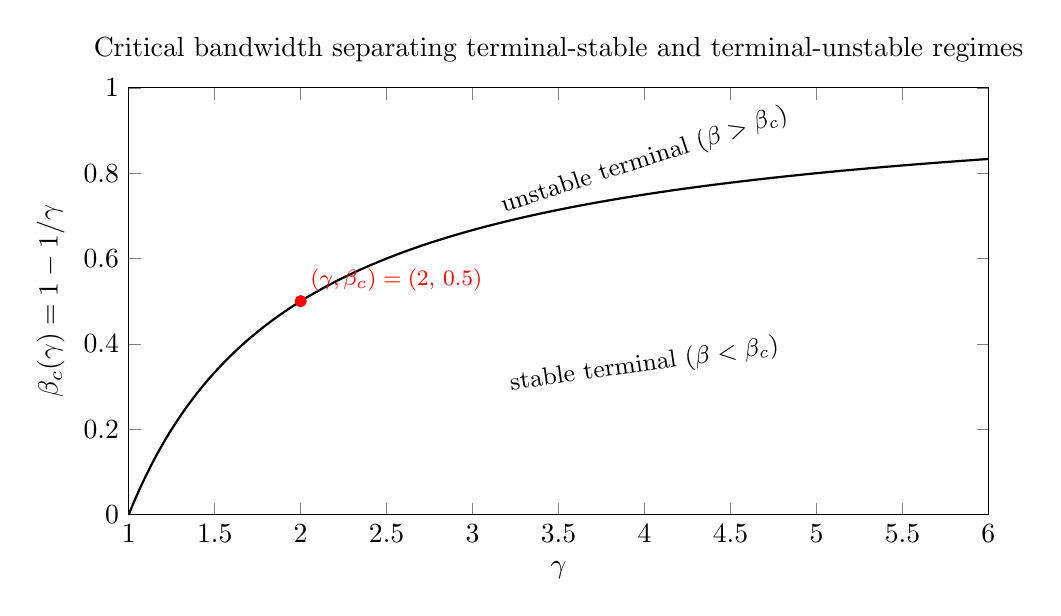
\begin{tikzpicture}
\begin{axis}[
  width=12.5cm,height=7cm,
  xlabel={$\gamma$}, ylabel={$\bwc(\gamma)=1-1/\gamma$},
  xmin=1,xmax=6, ymin=0,ymax=1,
  domain=1:6, samples=150,
  title={Critical bandwidth separating terminal-stable and terminal-unstable regimes},
]
\addplot[thick,black] {1-1/x};
\addplot[mark=*,mark size=2pt,red] coordinates {(2,0.5)};
\node[anchor=south west, red] at (axis cs:2,0.5) {\footnotesize $(\gamma,\bwc)=(2,\,0.5)$};
\node[rotate=18] at (axis cs:4,0.83) {\small unstable terminal ($\bw>\bwc$)};
\node[rotate=8] at (axis cs:4,0.35) {\small stable terminal ($\bw<\bwc$)};
\end{axis}
\end{tikzpicture}
\caption{The critical bandwidth curve $\bwc(\gamma)=1-1/\gamma$. Points above
the curve leave the symmetric terminal configuration transversely unstable
(as in the base model, which sits at the horizontal line $\bw=1$, always
above the curve); points below it stabilize the terminal point. The
special point $\gamma=2$ gives exactly $\bwc=1/2$, which reappears
independently in Section~\ref{sec:gamma2}.}
\label{fig:beta_c}
\end{figure}

\begin{warningbox}[This is a genuinely new phenomenon]
In the base model, the statement ``the terminal Pareto configuration is an
unstable saddle'' is a theorem with no free parameter to violate it. Once
the kernel has a tunable bandwidth, that statement becomes
\emph{conditional}: it holds only for $\bw>\bwc(\gamma)$. Sufficiently broad
kernels ($\bw<\bwc(\gamma)$, possible only when $\gamma>1$) make the fully
symmetric, undifferentiated population a locally stable outcome.
\end{warningbox}

% ============================================================
\section{Complete classification of the transverse profile}
\label{sec:classification}
% ============================================================

Equation~\eqref{eq:terminal_cases} only diagnoses the single terminal point.
The full trajectory sweeps $u=1+y^2$ from $1+h^2$ down to $1$, and we want
the sign of $\phib(u)$ on the whole interval $u\ge1$. This can be settled
completely using convexity.

\begin{lemma}
\label{lem:convexity}
For fixed $\bw,\gamma>0$, the function $\phib(u)=\bw\gamma u^{\gamma/2}-u-(\gamma-2)$
is strictly concave on $(0,\infty)$ if $\gamma<2$, strictly convex if
$\gamma>2$, and affine ($\phib(u)=(2\bw-1)u$) if $\gamma=2$.
\end{lemma}
\begin{proof}
Differentiate twice:
\[
  \phib''(u)=\bw\gamma\cdot\frac{\gamma}{2}\Big(\frac{\gamma}{2}-1\Big)u^{\gamma/2-2}.
\]
The prefactor $\bw\gamma\cdot\frac{\gamma}{2}>0$ and $u^{\gamma/2-2}>0$ for
$u>0$, so $\operatorname{sign}(\phib'')=\operatorname{sign}(\gamma/2-1)$,
which is negative for $\gamma<2$, positive for $\gamma>2$, and zero for
$\gamma=2$ (in which case direct substitution gives
$\phib(u)=2\bw u-u-0=(2\bw-1)u$ exactly).
\end{proof}

\begin{proposition}[Global sign structure of $\phib$]
\label{prop:global_sign}
Let $\gamma\ne2$. As $u\to0^+$, $\phib(u)\to-(\gamma-2)=2-\gamma$, and as
$u\to\infty$, $\phib(u)\to-\infty$ if $\gamma<2$ and $\phib(u)\to+\infty$ if
$\gamma>2$. Consequently there is exactly one crossing $u_c=u_c(\gamma,\bw)>0$
with $\phib(u_c)=0$, and:
\begin{itemize}[leftmargin=1.4em]
\item if $\gamma<2$: $\phib>0$ for $u<u_c$ and $\phib<0$ for $u>u_c$;
\item if $\gamma>2$: $\phib<0$ for $u<u_c$ and $\phib>0$ for $u>u_c$.
\end{itemize}
\end{proposition}
\begin{proof}
The limits follow directly from \eqref{eq:phi_beta}, since $u^{\gamma/2}$
grows slower than $u$ for $\gamma<2$ and faster for $\gamma>2$. For
$\gamma<2$, $\phib$ is strictly concave (Lemma~\ref{lem:convexity}), so its
superlevel set $\{u>0:\phib(u)\ge0\}$ is convex, i.e.\ an interval; it
contains points near $0$ (where $\phib\to2-\gamma>0$) but not arbitrarily
large $u$ (where $\phib\to-\infty$), so it is an interval of the form
$(0,u_c]$, giving exactly one crossing with the stated sign pattern. For
$\gamma>2$, $\phib$ is strictly convex, so its \emph{sub}level set
$\{u>0:\phib(u)\le0\}$ is an interval; it contains points near $0$ (where
$\phib\to2-\gamma<0$) but not arbitrarily large $u$ (where
$\phib\to+\infty$), giving the complementary sign pattern.
\end{proof}

Combining Proposition~\ref{prop:global_sign} with the physical constraint
$u\ge1$ (i.e.\ $y\in\R$) and the sign of $\phib(1)$ from
\eqref{eq:terminal_cases} yields the complete table:

\begin{center}
\renewcommand{\arraystretch}{1.35}
\begin{tabular}{@{}lll@{}}
\toprule
\textbf{Regime} & \textbf{Condition} & \textbf{Transverse profile on the trajectory ($u:1{+}h^2\to1$)}\\
\midrule
$\gamma\le1$ & any $\bw>0$ & stable far away $\to$ unstable near terminal\\
$1<\gamma<2$ & $\bw>\bwc(\gamma)$ & stable far away $\to$ unstable near terminal (as base model)\\
$1<\gamma<2$ & $\bw<\bwc(\gamma)$ & \textbf{stable everywhere} — no bifurcation for any $h$\\
$\gamma=2$   & $\bw>1/2$ & uniformly unstable, $\lsplit\equiv\frac{4\bw(2\bw-1)}{N}$\\
$\gamma=2$   & $\bw<1/2$ & uniformly \textbf{stable}, $\lsplit\equiv\frac{4\bw(2\bw-1)}{N}$\\
$\gamma>2$   & $\bw>\bwc(\gamma)$ & unstable everywhere (as base model)\\
$\gamma>2$   & $\bw<\bwc(\gamma)$ & \textbf{inverted}: unstable far away $\to$ stable near terminal\\
\bottomrule
\end{tabular}
\end{center}

\begin{warningbox}[The inverted regime is qualitatively new]
For $\gamma>2$ and $\bw<\bwc(\gamma)$, a population launched far enough from
the targets ($h>\sqrt{u_c-1}$) begins its descent in the \emph{unstable}
regime, yet the symmetric configuration \emph{re-stabilizes} as the
population approaches the targets. This is the exact opposite ordering from
every case in the base model, where instability only ever develops on
approach to the terminal point, never away from it.
\end{warningbox}

% ============================================================
\section{The exactly solvable case $\gamma=2$}
\label{sec:gamma2}
% ============================================================

At $\gamma=2$, $\phib(u)=(2\bw-1)u$ exactly (Lemma~\ref{lem:convexity}), so
by \eqref{eq:lsplit_beta} with $\gamma=2$ (hence $(1+y^2)^{(\gamma-4)/2}=(1+y^2)^{-1}$):
\begin{equation}
  \boxed{
  \lsplit\Big|_{\gamma=2}
  =
  \frac{4\bw}{N}(1+y^2)^{-1}(2\bw-1)(1+y^2)
  =
  \frac{4\bw(2\bw-1)}{N},
  }
  \label{eq:gamma2_exact}
\end{equation}
\emph{independent of $y$}. At $\gamma=2$ the transverse eigenvalue is
constant along the entire trajectory: the population is either uniformly
stable ($\bw<1/2$), uniformly unstable ($\bw>1/2$), or exactly marginal at
every point ($\bw=1/2$, $\lsplit\equiv0$). This matches
$\bwc(2)=1-\tfrac12=\tfrac12$ from \eqref{eq:beta_c}, confirming the two
independent computations agree.

% ============================================================
\section{Consistency check: the nonlinear reduced potential}
\label{sec:nonlinear}
% ============================================================

As in the base model, introduce the two-group order parameter $m\in[-1,1]$
with $x_\pm=\pm m$ and common height $y$, and
$r_\pm=\sqrt{(1\pm m)^2+y^2}$. The exact reduced potential is
\begin{equation}
  U(m,y)=-2\log\left[\frac{N}{2}\Big(e^{-\bw r_+^{\gamma}}+e^{-\bw r_-^{\gamma}}\Big)\right].
  \label{eq:Ured_beta}
\end{equation}
Write $u=1+y^2$ and $\psi(m)=(u+2m+m^2)^{\gamma/2}$, so that
$f(m)=e^{-\bw\psi(m)}+e^{-\bw\psi(-m)}$ and $U=-2\log(\tfrac{N}{2}f(m))$.

At $m=0$: $\psi(0)=u^{\gamma/2}$, and differentiating twice,
\[
  \psi'(0)=\gamma u^{\gamma/2-1},
  \qquad
  \psi''(0)=\gamma u^{\gamma/2-2}\big[(\gamma-2)+u\big].
\]
Applying $\frac{d^2}{dm^2}e^{-\bw\psi}\big|_0=e^{-\bw u^{\gamma/2}}\big[\bw^2\psi'(0)^2-\bw\psi''(0)\big]$
to both terms of $f$ (which are mirror images under $m\mapsto-m$, so their
second derivatives at $m=0$ coincide) gives
\begin{align}
  f''(0)
  &=
  2e^{-\bw u^{\gamma/2}}
  \Big[\bw^2\gamma^2 u^{\gamma-2}-\bw\gamma u^{\gamma/2-2}(u+\gamma-2)\Big]
  \nonumber\\
  &=
  2\bw\gamma\, e^{-\bw u^{\gamma/2}}u^{\gamma/2-2}
  \Big[\bw\gamma u^{\gamma/2}-u-(\gamma-2)\Big]
  \;=\;
  2\bw\gamma\, e^{-\bw u^{\gamma/2}}u^{\gamma/2-2}\,\phib(u).
  \label{eq:fpp0_beta}
\end{align}
Since $f(0)=2e^{-\bw u^{\gamma/2}}$ and $f'(0)=0$ by symmetry,
\begin{equation}
  \boxed{
  \left.\frac{\partial^2 U}{\partial m^2}\right|_{m=0}
  =
  -2\frac{f''(0)}{f(0)}
  =
  -2\bw\gamma\, u^{\gamma/2-2}\phib(u)
  =
  -N\lsplit(y),
  }
  \label{eq:consistency_check}
\end{equation}
using \eqref{eq:lsplit_beta}. This is exactly the same relation as in the
base model: the linear stability calculation and the curvature of the exact
nonlinear reduced potential agree for every $\bw$, confirming the
derivation is internally consistent.

% ============================================================
\section{Beyond two targets}
\label{sec:general_geometry}
% ============================================================

For a general configuration, \eqref{eq:M_tau_beta} defines the transverse
tensor $\Lsplit(\bx)=M(\bx)-\tau(\bx)I$ everywhere; its eigenvalues
$\lambda_a(\bx)=\mu_a(\bx)-\tau(\bx)$ (where $\mu_a$ are the eigenvalues of
$M$) determine the bandwidth-dependent bifurcation set
\begin{equation}
  \boxed{
  \mathcal B_{\bw}=\{\bx:\lambda_{\max}(\bx)=0\}.
  }
  \label{eq:bifurcation_set}
\end{equation}

\subsection{Three targets}
\label{sec:three}

For $\ba_{1,2}=(\mp b,0)$ (recall: $b$ is the geometric half-spacing, not the
bandwidth) and $\ba_3=(0,e)$, with $d_e=\sqrt{b^2+y^2}$, $d_3=|y-e|$, the
same substitution $\gamma d_i^\gamma\mapsto\bw\gamma d_i^\gamma$ applied to
the base model's three-target formulas gives
\begin{align}
  \boxed{
  \lambda^x_{\rm split}(y)
  =
  \frac{\bw\gamma}{N}
  \left\{
  2d_e^{\gamma-4}\Big[\bw\gamma b^2 d_e^{\gamma}-(\gamma-2)b^2-d_e^2\Big]
  -
  d_3^{\gamma-2}
  \right\}
  }
  \label{eq:three_x_beta}\\[6pt]
  \boxed{
  \lambda^y_{\rm split}(y)
  =
  \frac{\bw\gamma}{N}
  \left\{
  2d_e^{\gamma-4}\Big[\bw\gamma y^2 d_e^{\gamma}-(\gamma-2)y^2-d_e^2\Big]
  +
  d_3^{\gamma-2}\Big[\bw\gamma d_3^{\gamma}-\gamma+1\Big]
  \right\}
  }
  \label{eq:three_y_beta}
\end{align}
The central target's contribution to the left--right (lateral) mode is still
the strictly stabilizing term $-\dfrac{\bw\gamma}{N}d_3^{\gamma-2}$: a
third, on-axis target suppresses the left--right instability regardless of
bandwidth, though the \emph{size} of that suppression now scales with
$\bw$ as well.

% ============================================================
\section{Why bandwidth is not just another population size}
\label{sec:beta_vs_N}
% ============================================================

In the base model, $N$ enters every rate as an overall $1/N$ factor and can
be absorbed into a rescaled clock $\tau=t/N$ (with $\sigma_{\rm eff}=\sigma\sqrt N$
in the stochastic theory); it never moves the deterministic bifurcation set.
Bandwidth does not have this property: $\bw$ appears \emph{both} as an
overall prefactor \emph{and} inside $\phib(u)=\bw\gamma u^{\gamma/2}-u-(\gamma-2)$,
where it competes against the fixed terms $-u-(\gamma-2)$. This is precisely
why $\bw$ can relocate, remove, or invert the crossing $u_c(\gamma,\bw)$
(Section~\ref{sec:classification}), while $N$ can only change how fast the
trajectory moves through a bifurcation structure that is already fixed by
$(\gamma,\bw)$ alone.

\begin{keybox}[Summary]
$(\gamma,\bw)$ jointly and non-separably determine \emph{where} (and even
\emph{whether}) the transverse instability occurs; $N$ and the noise
amplitude $\sigma$ only determine \emph{how quickly} and \emph{how visibly}
that instability, once present, develops into a macroscopic fan.
\end{keybox}

% ============================================================
\section{Conclusion}
\label{sec:conclusion}
% ============================================================

Introducing an explicit bandwidth $\bw$ into the kernel, $p(d)=e^{-\bw d^\gamma}$,
preserves the entire analytic structure of the base model — the same
gradient-flow derivation, the same collective transverse tensor, the same
correspondence between the linear eigenvalue and the curvature of the exact
nonlinear potential — under the single, uniform substitution
$\gamma d^{\gamma}\mapsto\bw\gamma d^{\gamma}$ inside every stability
bracket, with $\gamma\mapsto\bw\gamma$ as the overall rate prefactor.

What changes qualitatively is the bifurcation structure itself. The
base model's theorem that ``the terminal Pareto configuration is always
transversely unstable'' is a special case, true only along the line
$\bw=1$ in a two-dimensional $(\gamma,\bw)$ phase plane whose boundary is
the critical curve $\bwc(\gamma)=1-1/\gamma$. Crossing that curve — by
broadening the kernel rather than by changing its shape exponent $\gamma$ —
can stabilize the terminal configuration entirely, or, for $\gamma>2$,
invert the order in which stability is lost and regained along the
trajectory. The exponent $\gamma=2$ remains special: there the transverse
eigenvalue collapses to the $y$-independent constant
$\lsplit=\tfrac{4\bw(2\bw-1)}{N}$, and the critical curve passes through
the clean point $\bwc(2)=\tfrac12$.

The single cell ($N=1$) obeys a different, and in some ways sharper, story.
Its stability function $\psi(u)=u+(\gamma-2)$ never involves $\bw$ at all —
bandwidth can only rescale how fast a single cell's stability or
instability plays out, never whether it occurs — and its threshold sits at
$\gamma=1$, not $\gamma=2$ or $\bwc(\gamma)$. Convexity of the single-cell
cost promotes this local threshold to a global one: for $\gamma\ge1$ every
trajectory, from any starting point, converges to the shared compromise;
for $\gamma<1$ every off-axis trajectory instead reaches a single archetype
exactly, in finite time. Bandwidth reshapes the population's bifurcation
structure precisely because the population's normalizing sum $S_i$
reintroduces $\bw\gamma d_i^\gamma$ into the collective eigenvalue — the
very term a single cell's logarithm cancels away.

\end{document}
